\chapter{Power Markets And The Role of Flexibility Management: A Qualitative Analytical Framework}
\chaptermark{Market regimes}
\label{ch:market}
\textit{This chapter aims at offering a comparative view on different power market regimes, based on which an analytical framework can be established. Such a framework offers technology vendors the fundamental for qualitatively analyzing the opportunities of flexibility management in a given market context. By mapping a list of maturely existing power markets worldwide, we extract some key attributes of power market structures that have impacts on value of flexibility management.}

\section{Motivation for a framework over various power market regimes}

Started in the 1980s and facilitated in 1990s, liberalization of power markets has been the mainstream worldwide \cite{Srivastava2011,Ranci2013,Vagliasindi2013}. Nowadays, liberalized power markets have been maturely established in many economies especially in developed countries. 
However, since different preconditions exist in these economies including historical, political and climatic reasons, structures of these power markets tend to be very heterogeneous. %Moreover, with development of technologies, power markets face pending or undergoing restructuring, make them a rapidly changing field of the economy. \cite{Ziel2015}
This brings great challenges to companies that pursue cross-regional or even global footprint, since business models of flexibility management as well as their feasibility and performance depend extensively on the power market structure. Compared to other stakeholders that are interested in flexibility management such as utilities, technology vendors are particularly prone to international expansion. This is not only because they have fewer regulatory barriers, but also because firms with higher research and development (R\&D) intensity have stronger motivation for expanding geographic boundaries to mitigate market risks and seek growth opportunities \cite{Brouthers2007}.

Therefore, in this chapter we map the taxonomy of power markets with particular focus on characteristics related to flexibility management, in order to provide a guidance for technology vendors to initiate analysis while facing an unfamiliar power market.

Such a global view is established by generalizing and comparing market regimes in different systems that are listed in Table \ref{tab:markets}. We will name a few of them as typical examples while discussing each structural attribute. However, it shall be noted that the goal of this chapter is not to provide comprehensive analysis on each of the system. With on-going restructures, market regime in each system is such a dynamic manner that is constantly evolving over time. Taking the electricity market in Great Britain (GB) as example, it had been operating in the model of power pool for over 10 years before it reformed to a power exchange arrangement in 2001 \cite{Rebours2009,FrontierEconomics2016,ofgem_m}, and in a more recent restructuring in 2014 they established the capacity market that does not exist there before \cite{ofgem_cm}. 

Nevertheless, the global framework will remain generally stable regardless of adjustments in individual markets. This again reveals the importance of an analytical framework facing such a fast-changing area. Using the same example in GB, readers can immediately identify new opportunities incident to the introduction of capacity market by referring to Section \ref{sec:CM}.


\begin{table}[h!]
	\small
	\centering
	\begin{tabular}{L{5cm} l l l}
		\hline
		\hline
		\textbf{System} & \textbf{Abbreviation} & \textbf{Country} & \textbf{Main Reference} \\
		\hline
		\hline
		PJM Interconnection & PJM & US & \cite{Rebours2009,Srivastava2011,Cochran2013,EllisonJ.F.TesfatsionL.S.LooseV.W.Byrne2012,Gilstrap2015,Brown2015,Borenstein2015,PJM_web,PJM2017b,PJM2017c}\\
		\hline
		New York ISO & NYISO & US & \cite{Cochran2013,EllisonJ.F.TesfatsionL.S.LooseV.W.Byrne2012,Gilstrap2015,Borenstein2015,NYISO_web}\\
		\hline
		Midcontinent ISO\footnote{Formerly named Midwest ISO}& MISO & US \& Canada& \cite{EllisonJ.F.TesfatsionL.S.LooseV.W.Byrne2012,Gilstrap2015,Borenstein2015,MISO_web}\\
		\hline
		ISO New England & ISO-NE & US & \cite{EllisonJ.F.TesfatsionL.S.LooseV.W.Byrne2012,Gilstrap2015,Borenstein2015,ISO_NE_web}\\
		\hline
		California ISO & CAISO & US& \cite{Rebours2009,EllisonJ.F.TesfatsionL.S.LooseV.W.Byrne2012,Gilstrap2015,Borenstein2015,CAISO_web}\\
		\hline
		Southwest Power Pool & SPP & US & \cite{EllisonJ.F.TesfatsionL.S.LooseV.W.Byrne2012,Gilstrap2015,Borenstein2015,SPP_web}\\
		\hline
		Electric Reliability Council of Texas & ERCOT & US & \cite{Srivastava2011,EllisonJ.F.TesfatsionL.S.LooseV.W.Byrne2012,Brown2015,Gilstrap2015,Borenstein2015,ERCOT_web}\\
		\hline
		Ontario Independent Electricity System Operator& IESO/ Ontario& Canada & \cite{Cochran2013,Brown2015,Ontario_web}\\
		\hline
		Alberta Electric System Operator & AESO/Alberta & Canada &  \cite{Brown2015,Alberta_web}\\
		\hline
		National Electricity Market (Australia) & NEM & Australia & \cite{Srivastava2011,Brown2015,AEMO2010,AEMO2015a}\\
		\hline
		National Electricity Market of Singapore & NEMS & Singapore & \cite{Brown2015} \\
		\hline
		Germany\footnote{Referring to territories of Tennet, Amprion, 50 Hertz, TransnetBW under the regulation of Bundesnetzagentur (BNA) with large volume of electricity traded OTC and on power exchange, EPEX SPOT. } & DE & Germany & \cite{FrontierEconomics2016,Wartsila2014,ConsentecGmbH2014,Deloitte2015} \\
		\hline
		Single Energy Market (Ireland) & SEM/ Ireland & Ireland & \cite{FrontierEconomics2016,Cochran2013}\\
		\hline
		Great Britain\footnote{Referring the territory of the TSO, National Grid, under the regulation of Office of Gas and Electricity Markets (ofgem) with large volume of electricity traded OTC and on power exchange, APX Power UK and N2EX .} & GB & Great Britain & \cite{Rebours2009,FrontierEconomics2016,ofgem_cm,ofgem_m,EnergyUK2017} \\
		\hline
		Other European Markets & - & - & \cite{FrontierEconomics2016}\\
		\hline
		\hline
	\end{tabular}
	\caption{List of markets involved in this study} \label{tab:markets}
\end{table}

In Chapter \ref{ch:introduction}, we identify three applications of flexibility management in wholesale markets, including:

\begin{itemize}
	\item \textbf{Arbitrage in energy market}, and
	\item \textbf{Frequency control in ancillary services market}, and
	\item \textbf{Supply adequacy in capacity market}. 
\end{itemize}

Correspondingly, we systemically investigate how the feasibility of these applications is influenced by different market regimes, i.e. structure of energy/ ancillary service/ capacity markets, in the reminder of this chapter. Unlike many other studies comparing different market structures, we do no analyze the full rationale behind the market design nor their comprehensive merits and drawbacks. Instead, we are only focused on the differences themselves and their direct impacts on value of flexibility management, which shall be sufficient for our study.


~\newpage

\section{Flexibility management in energy market}
\sectionmark{Energy market}
We first focus on the wholesale energy market as it constitutes the central transaction platform in power market \cite{Cochran2013}. 

According to the principle of economics, in a competitive market price shall act as an effective signal to coordinate the relationship between supply and demand. Reflected in energy market, if the market is well-designed, price volatility will increase due to lack of flexibility and in turn become a incentive to encourage participation of new flexibility sources, as introduced in Chapter \ref{ch:introduction}. However, it is not always the case in reality since power market design has additional concerns for physical, and political reasons. Moreover, since market design is likely to lag behind technological development, some legacy rules tend to create barriers for new technologies even if they may be favored in those physical, economic and political aspects.

Therefore, although energy arbitrage that can absorb energy in supply surplus and release energy in supply shortage is theoretically beneficial to power systems, it is not always feasible depending on market rules. 

\subsection{Market model: Power pool vs. power exchange}

First of all, it is worthwhile to point out the difference  between power pool and power exchange, since they represent two fundamentally distinct approaches of power market organization. 

\begin{figure}[h!]
	\centering
	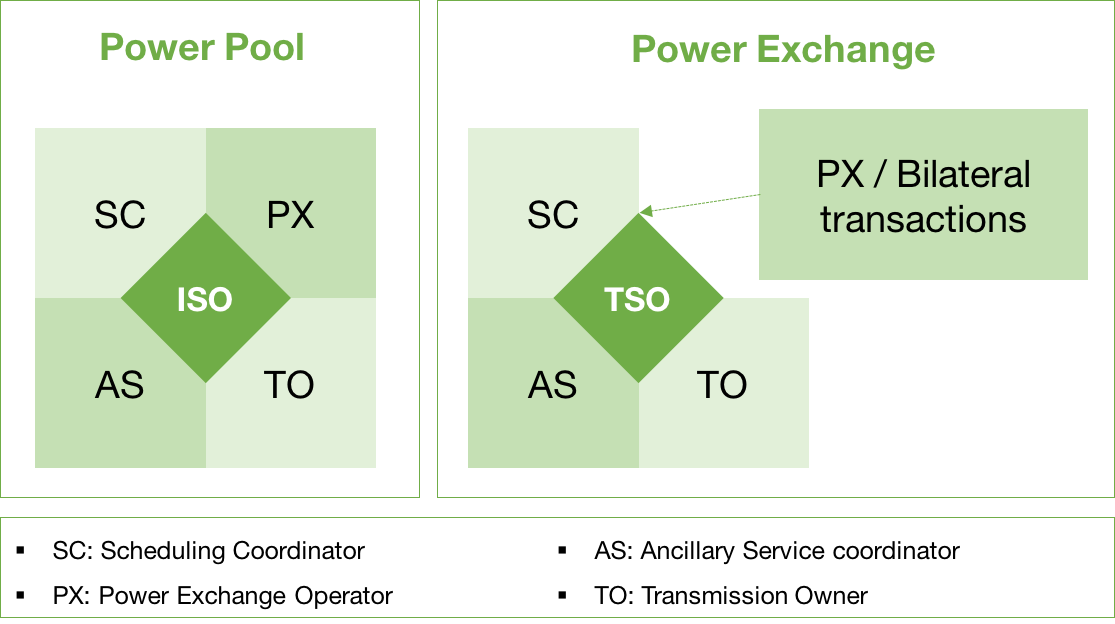
\includegraphics[width=0.95\linewidth]{Figures/PowerPoolExchange}
	\caption{Illustration of difference between power pool and power exchange}
	\label{fig:pppx}
\end{figure}

As shown by Figure \ref{fig:pppx}, in the model of power pool, all the structural components of power markets are integrated and coordinated by a single entity who is both market operator and system operator  \cite{Srivastava2011,Barroso2005}. Since scheduling is an integral part of the power market, schedules are determined through one single market gateway, and the market are cleared abiding by limits of physical deliveries.  
In a power pool, ISO seeks to minimize the system total production cost through a centralized unit commitment to fulfill demands economically. Generators must follow the commitment schedule and the dispatch instructions issued by the ISO to receive the market whole side payments \cite{Kardakos2013}. Market activities are mainly on the generation-side, while demands are collected just as input of ISOs' optimization. Players on the demand-side are usually not able to participate in the market directly unless specific measures are implemented.

In contrast, with the model of power exchange, while a transmission system operator is still responsible for scheduling coordination, ancillary service provision and transmission system operation, power transactions are made through a power exchange organized by a third-part or bilateral contracts. Therefore, a market participant is able make electricity transactions in more than one market gateways. As a matter of fact, power exchanges are mostly voluntarily established and evolved from the bilateral contract model \cite{Barroso2005}. The system operator usually have no direct control on the power exchanges and its role is limited to the physical aspect of maintaining system security. Each producer is responsible for self-scheduling its own units with a decentralized price-based unit commitment \cite{Kardakos2013}.


Examples of energy markets organized in power pool:
	\begin{itemize}
		\item Most markets organized by ISOs in North America such as PJM, NYISO, Alberta, etc.
		\item Australia's NEM
		\item Ireland's SEM.
	\end{itemize}

Examples of energy markets organized in power exchange
	\begin{itemize}
		\item most markets in European countries such as Germany, Nord Pool, GB etc.
		\item CAISO in the US
	\end{itemize}

\subsubsection{Implications for flexibility management}
In power exchange, the participation from supply-side and demand-side is generally symmetric and offers/bids are usually in the single form of price-quantity pairs. The physical realization of delivery is unbundled  from market activities and is not concerned by market operators. This allows great freedom for flexibility players to participate in the market, regardless of whether the flexibility comes from supply- or demand- side or mixed, and which technologies are employed. 

In power pool, however, generators are usually required to submit complex unit offers including physical information of resources, e.g., unit start-up and shut-down procedures, minimum-up/down time constraints, min/max power output restrictions, ramp-rate limits, transmission limits etc. \cite{Kardakos2013}, and participation from demand-side is generally limited. Therefore, with bundling physical and market activities, participation of flexibility is extensively under control of power pool operators. Being recognized as a generation resource or special market gateway for demand-side participation is necessary prerequisite for a new flexibility resource to directly participate in markets. Otherwise, it would be only limited to behind-the-meter applications where some flexibility resources such energy storage can complement with existing resource or load to adjust a player's position in market. In this way, the operation of flexibility might not be optimal and aggregation is impossible. In addition, due to the strong position of power pool operators, it is less likely for players to gain market power than in power exchange.

Overall, there are much more limits for market participation of flexibility management in power pool than in power exchange. Technology vendors need to pay more attentions to market rules and regulatory environment for business planning in power pool than in power exchange. 

\subsection{Marketplaces}

In most regions, the energy market consists of several marketplaces along the timeline, as shown by \ref{fig:energy-marketplaces}.

\begin{figure}[h!]
	\centering
	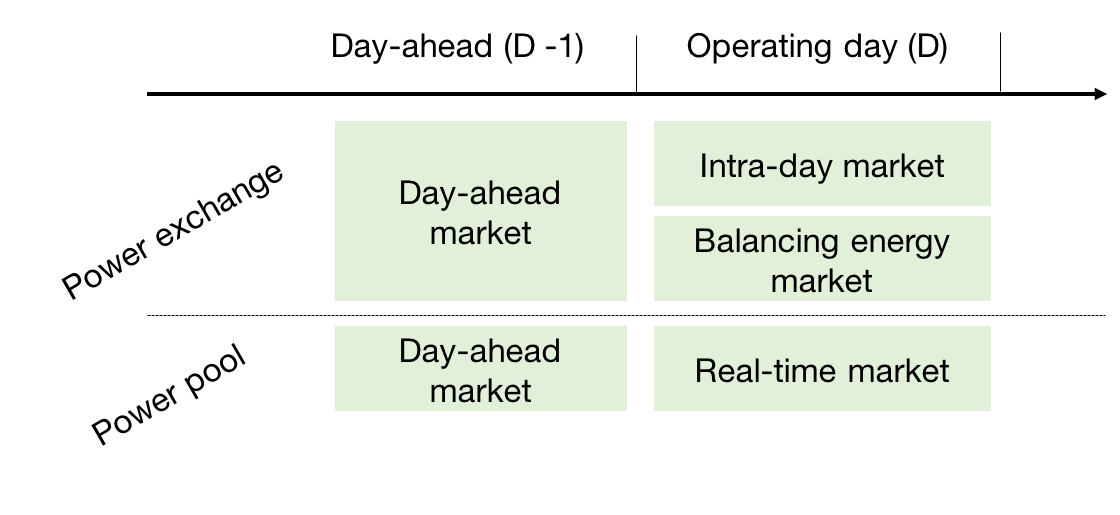
\includegraphics[width=0.95\linewidth]{Figures/EnergyMarketplaces}
	\caption{Typical marketplaces in wholesale energy market}
	\label{fig:energy-marketplaces}
\end{figure}

In markets organized with power exchange model, large volumes of energy are usually traded in day-ahead (DA) market. Intra-day (ID) market, which can be viewed as an extension of day-ahead spot market bringing gate closure near delivery, become an usual measure to mitigate increasing needs of real-time balancing operations, as introduced in Chapter \ref{ch:introduction}. All deviations from the commitment scheduled by DA and ID markets requires balancing energy delivery that is coordinated by system operators and are settled through a third marketplace, often named balancing energy market. In most cases, balancing energy market is purely for settlement without any explicit trading activities.

Slightly different arrangements are adopted in power pools. Since delivering balancing energy is responsible by same entity who operates the energy markets, real-time markets are used for settlements of both post-DA scheduling adjustments and balancing operations.

The three-settlement market is the European Union target electricity model \cite{EuropeanCommission2016} so has been implemented in most European energy markets such as Germany, France, Denmark, GB, Italy, Spain, etc.  Two-settlement market, on the other hand, is a common practice in North America  \cite{Cochran2013}.

%\subsubsection{Implications for flexibility management}
Generally, arbitrage in DA market is less favorable for emerging flexibility players, due to relative low volatility and dominance of large conventional generation companies. Flexibility management shall gain more advantage in market closer to delivery due to its comparative competence of fast response and operations to conventional generators. 

Nonetheless, participation in any marketplace to perform arbitrage is potentially profit-making. Therefore, identifying which marketplaces exist and whether they are accessible is a necessary step for valuing the opportunities of flexibility management.

\subsection{Pricing scheme}
If a marketplace is accessible for flexibility players, a further concern would be the profitability of arbitrage. Since arbitrage is essentially a game played with prices, the pricing scheme is of most importance, which is however varying in details among different markets.

\subsubsection{Nodal pricing vs. zonal pricing}
With nodal pricing scheme, prices at each transmission bus (node) are different. On the contrary, uniform pricing scheme applies same price everywhere in the whole control area. Zonal pricing as a trade-off between these two schemes, use the same price in a particular zone including a bundle of nodes.

Nodal pricing internalizes network congestion in price formation. If congestion restricts lowest-cost electricity being transmitted to a particular location, electricity with higher cost but no congestion is dispatched and consequently price at that location will rise. Benefits of nodal pricing is affirmative \cite{Wang2015} but it is not harder to be implemented, especially in markets arranged in power exchange where market operator have no insight into the physical system\footnote{In these regions, it is possible to be implemented nodal pricing in balancing markets that is coordinated by physical system operators, as illustrated by a research project \cite{Ecogrid}. However, we did see any large-scale practice in reality. Besides, balancing markets are not the target markets for arbitrage.}. 

Nodal pricing is adopted in many systems in North America, such as PJM, CAISO, NYISO, ISO-NE etc., using a mechanism named locational marginal price (LMP) model. Zonal pricing is used in Australia's NEM and other energy markets organized in power exchange model. 

Since nodal pricing incorporates the consideration of congestion. The value of T\&D congestion relieves are theoretically able to be partially captured by arbitrage, especially using some flexibility technologies that are easier to be deployed with smaller scale in particular locations such as batteries. However, for aggregator, nodal pricing increases the operational complexity for them.

\subsubsection{Resolution}
Since RES generation may vary significantly in a short time interval so as the residual load, higher resolution of pricing can better represent the need for flexibility. Emerging flexibility solutions with faster response and higher ramp rate shall gain advantages with higher pricing resolution in theory. However, it shall be noticed that the pricing and dispatching time interval is often different with the settlement interval. For example, the real-time markets in PJM has 5-min pricing resolution but settlement of energy delivery is accounted in hourly resolution \cite{PJM2017}. In such an arrangement, arbitrage following the original price signals may be activated for price differences within a settlement interval and thus brings no revenue. 


\section{Flexibility management in ancillary service market}
\sectionmark{Ancillary service market}
Among all ancillary services, this thesis is particularly focused on frequency control services that are used to tackle imbalance between supply and demand, as introduced in Chapter \ref{ch:introduction}. Frequency control services are usually the most costly among all ancillary services and relying on services provision from market players, while there are usually no markets for other ancillary services such as voltage support, loss compensation, black start etc \cite{Rebours2009,Cochran2013}. 

In different regimes, there exist many differences regarding how frequency control services are defined, procured and operated, as well how the cost is allocated and recovered. Understanding these differences allows technology vendors know which services can be provided using flexibility and to whom they can sell flexibility solutions.

\subsection{Terminology for frequency control services}

Different terminologies used in different power jurisdictions may easily lead to confusion while comparison between different regimes is to be made. Different terms are often used to refer to the same service, while in some instances the similar terms may refer to two disparate services in different regimes. For example, secondary control reserve (SCR) and automatic frequency restoration reserve (aFRR) are interchangeable concepts. On the opposite, primary reserve in North America is often used to distinguish services from supplementary reserve, while it is closer to the concept of tertiary reserve rather than primary reserve used in Europe.

Generally, these terminologies can be classified into two scream as they are following the guidance of service definitions from the Federal Energy Regulatory Commission (FERC) and the Union for the Coordination of the Transmission of Electricity (UCTE). According to the functioning mechanism\footnote{ PCR refers to response activated locally by a speed governor fitted in generator. SCR is activated by a centralized control signal named automatic generation control (AGC) signal. TCR follows manual orders from system operators \cite{EllisonJ.F.TesfatsionL.S.LooseV.W.Byrne2012}. }, terminologies in these two systems can be mapped into a a comparison framework show by Table \ref{tab:term}.

\begin{table}[h!]
	\footnotesize
	\centering
	\begin{tabular}{L{3cm} L{3cm} | L{3cm} L{3cm}}
		\hline
		\hline
		\textbf{UCTE terms} &  \textit{Equivalents} & \textbf{FERC terms} &  \textit{Equivalents} \\
		\hline
		\hline
		Primary control reserve (PCR) & Frequency containment reserve (FCR) & Frequency response & \\
		\hline
		Secondary control reserve (SCR) & Automatic frequency restoration reserve (aFRR) & Frequency regulation & \\
		\hline
		\multirow{3}{3cm}{Tertiary control reserve (TCR)}
		  & \multirow{3}{3cm}{Manual frequency restoration reserve (mFRR)} & Spinning reserve & Synchronous reserve \\
		  \multirow{3}{3cm}{}& \multirow{3}{3cm}{}& Non-spinning reserve & Non-synchronous reserve/ Quick-start reserve \\
		  \multirow{3}{3cm}{}&\multirow{3}{3cm}{} & Supplemental reserve & Replacement reserve \\
		  \hline
		  \hline
	\end{tabular}
\caption{Terminology for frequency control reserves in various regimes \cite{Rebours2009,EllisonJ.F.TesfatsionL.S.LooseV.W.Byrne2012,Wang2015}}\label{tab:term}
\end{table}

It shall be noted that in terms of activation time, UCTE has specifically defined that:

\begin{itemize}
	\item Primary reserve shall be automatically activated within 30s;
	\item Secondary reserve need to be completely delivered within 15 minutes; 
	\item Tertiary reserve shall start within 15-20 minutes after received the order from system operators.
\end{itemize}

In contrast, the time framework for each service category is not aligned among markets in North America \cite{EllisonJ.F.TesfatsionL.S.LooseV.W.Byrne2012}, but generally, activation time frequency regulation is comparable to a in-between state of primary and secondary control reserve. 

In addition, there are no markets for frequency response in North America \cite{EllisonJ.F.TesfatsionL.S.LooseV.W.Byrne2012} that is equivalent to primary control reserve in Europe.

Generally, new flexibility solutions have advantages for services with shorter activation time and shorter duration compared to service providers using conventional generations. Therefore, frequency control services can be roughly ranked in accordance with the extent to which they are favored for emerging technologies, from most to lest: primary, secondary and tertiary. However, this is very case-specific depending on characteristics of specific technology and market, so is not discussed in details here.

\subsection{Procurement and cost allocation}

Usually, markets for frequency control services involve trading for two commodities, i.e. capacity and energy, as shown by Figure \ref{fig:FCR_market}. 

\begin{figure}[h!]
	\centering
	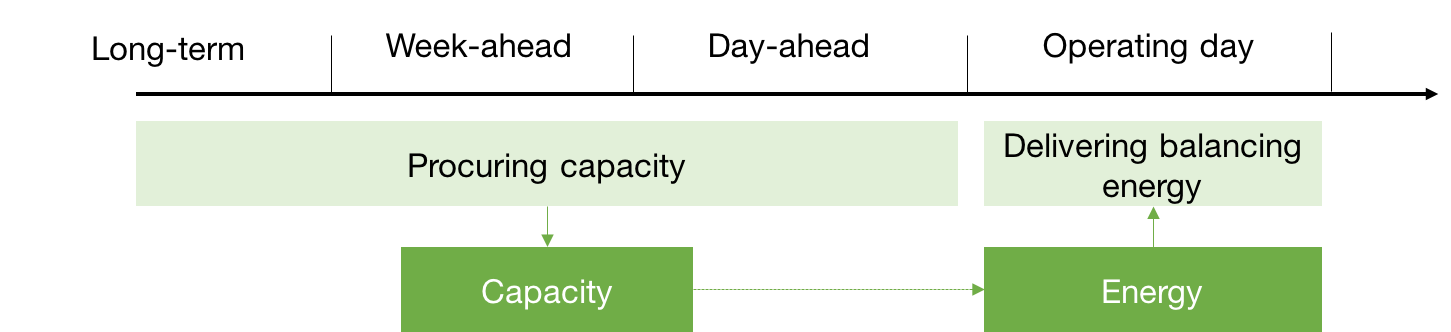
\includegraphics[width=0.95\linewidth]{Figures/FCR_market}
	\caption{Illustration of markets and activities related to frequency control services}
	\label{fig:FCR_market}
\end{figure}

Capacity refers to a commitment that service provide make to system operators, which shall be ready to be dispatch for real-time operations.  Requirement for capacity is determined by system operator and procured ahead of real-time operation. Specifically, in the continental European synchronously interconnected system, a total PCR of 3000 MW need to be provided According to the rules of the European Network of Transmission System Operator (ENTSO-E), while amounts of necessary SCR and TCR capacity are dimensioned by each TSO \cite{ENTSO-e_handbook}. For instance, in Germany, TSOs run a quarterly assessment process to dimension the provision of SCR and TCR for next three months (in March, June, September and December \cite{ConsentecGmbH2014}. In North America, ISOs determine the need for reserve capacity by conducting their own \textit{reliability assessment} processes, which take place after gate closure of day-ahead market and before each operating hour\cite{EllisonJ.F.TesfatsionL.S.LooseV.W.Byrne2012}. 

Energy is what services providers actually deliver to the system upon activation by system operators. The amount of energy is determined based on the real-time physical needs for grid balancing.

The acquisition and settlement process for the frequency control capacity and energy also varies amongst different market regimes.

Generally, two models are identified. We name them as centralized procurement and decentralized procurement respectively; see Figure \ref{fig:FCR_market-model}.

\begin{figure}[h!]
	\centering
	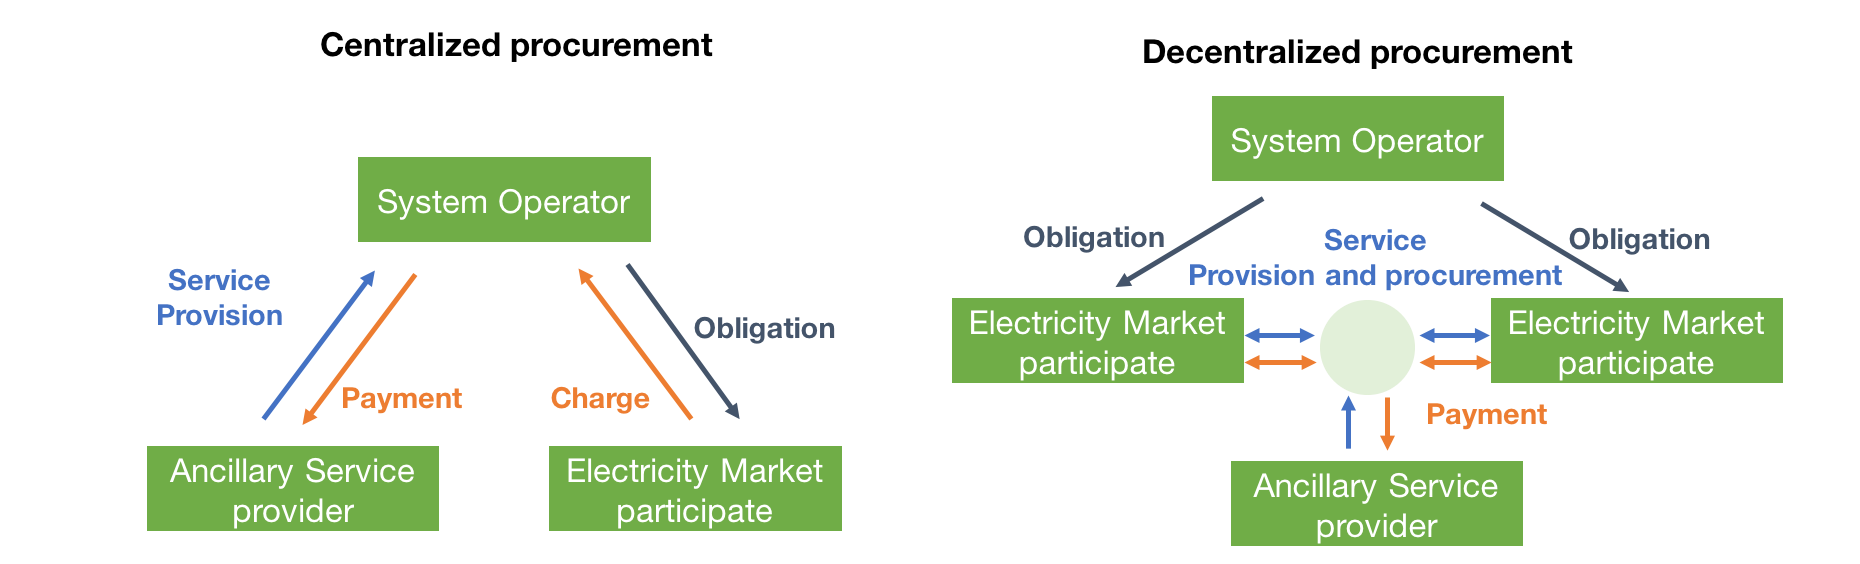
\includegraphics[width=0.95\linewidth]{Figures/FCR_market_model}
	\caption{Two models for procurement and cost allocation of frequency control services}
	\label{fig:FCR_market-model}
\end{figure}

In the centralized model, the system operator is designated as the single buyer \cite{Rebours2009}. System operators (SO) will either organize auctions in short term ahead of the operating day, e.g. German TSOs organize weekly-ahead auctions for SCR and day-ahead auctions for TCR \cite{ConsentecGmbH2014}, or seek long-term bilateral contract with service providers, e.g. Australian Energy Market Operator (AEMO) uses this approach to organize ancillary services in NEM \cite{AEMO2015}. On the other hand, SOs need to recover costs incurred by charge entities with obligation. In different markets and for disparate services, obligations are assigned in various ways. For example, costs for energy of frequency control services in Germany and for regulation reserve in Australia are recovered from entities who violate their commitments determined in energy markets, while costs for capacity of frequency control services in Germany and for contingency reserve (similar to PCR) in Australia are socialized among all market participate. 

Decentralized model is adopted by ISOs in North America. In this model, ISOs allocate requirements for reserve capacity to market players according to their servicing loads to the system total load \cite{Rebours2009,EllisonJ.F.TesfatsionL.S.LooseV.W.Byrne2012,PJM2017b}. Market players have to fulfill their own obligations through self-supplied reserve, through bilateral contract with other market participants, and/or through purchases of reserve in some form of reserve market organized by ISO \cite{EllisonJ.F.TesfatsionL.S.LooseV.W.Byrne2012}. In this way, market participants in the power market are put into competition for procuring frequency control service. Examples using this model include all seven ISOs in the US.

Flexibility solutions can be employed for provision of frequency control services in both arrangements and for fulfilling obligations. However, while provision and obligation fulfillment are symmetric in the decentralized approach, there might be asymmetry in the centralized approach with SOs standing in-between. 

\subsection{Frequency control product design}
Further to those higher distinctions, attentions shall necessarily be paid to some key details regarding how the frequency control service as products are designed. These designs will significantly affect the feasibility and profitability of certain technologies providing frequency control services. Without mentioning too many technological specifications, we discuss only three points here. 

First of all, pre-qualifications of resources to provide each service shall be understood without any doubts.

Second, frequency control services are sometimes divided into up and down services. Up services mean there are generation shortage and injection of energy or reduction of demand are required. On the contrary, down services refer to situations where more demand or less generation is needed. Separate markets for these two types of services would allow more choices for flexibility players to make optimal offers in accordance of the technological characteristics of their flexibility resources.

Finally, it is of a concern how automatic frequency control signals are engineered. For example, an energy storage device that does not generate energy will favor a signal that is energy-neutral to it, i.e. the state of charge of the device cam come back to its initial value after a period of operation.

Overall, impact of product designs is a technical issue and will be further discussed in Chapter \ref{ch:cases}.

\section{Flexibility management in capacity market}
\sectionmark{Capacity Market}
\label{sec:CM}
As has been introduced, capacity market is not a common practice in all regions, which classifies markets to ``energy-only market" and ``market with capacity obligation" (or simply`` capacity market"). The impact of capacity market on flexibility management comes from explicit and implicit aspects. 
\subsubsection{Examples}
Market with capacity

Alberta transformed to capacity market, approved in 2016 and expected in 2020.


\section{Aggregator and demand side participation}



\section{Summary and the analytical framework}


Figure



Power exchange vs. power pool

The power exchange is a centralized market that usually uses simple offers/bids in the form of price-quantity pairs. The market operator (MO) solves a convex linear programming (LP) problem on an hour-by-hour basis to match the supply offers with the demand bids and determines the market clearing price without taking into account any technical aspects constraining the operation of the generating units or the transmission system. In a power exchange, the role of system operator (SO) is limited to preserving the system security, while each producer is responsible for self-scheduling his own units by solving a decentralized price-based unit commitment (PBUC).

On the other hand, a power pool is a centrally organized market that usually uses complex unit offers and the independent system operator (ISO, who usually acts both as MO and SO) solves a non-convex optimization problem, where a simultaneous 24-hour co-optimization of energy and reserve resources is performed under a large set of unit and system constraints (e.g., unit start-up and shut-down procedures, minimum-up/down time constraints, min/max power output restrictions, ramp-rate limits, transmission limits etc.). In a power pool, the objective of the ISO is the minimization of the system total production cost through a centralized unit commitment. The producers must follow the commitment schedule and the dispatch instructions issued by the ISO in exchange of the make-whole side payments that guarantee that they will fully recover their total operating costs.

